% !TEX program = pdflatex
% =============================================================================
% Mirroring the Scene Flips the Score: Causal Controls for Directional
% Language Grounding
%
% Single-file source. Only references.bib and figures/ are external.
% Section order: Introduction, Related Work, Audit Design, Base-Frame Response,
% Directional Completion, Symmetric Scene, Discussion, Limitations, Conclusion,
% references, Appendix A.
% =============================================================================

% Compile main.tex from this directory (or latexmk -cd). For an RA-L submission,
% place the official ieeeconf.cls from PaperCept here. IEEEtran is a local preview fallback only.
\IfFileExists{ieeeconf.cls}{%
  \documentclass[letterpaper,10pt,conference]{ieeeconf}%
}{%
  \documentclass[letterpaper,10pt,conference]{IEEEtran}%
}

\newif\ifanonymous
\anonymousfalse % Switch to \anonymoustrue for a double-blind review submission.

\IEEEoverridecommandlockouts % <--- MUST KEEP THIS
\usepackage{amsmath,amssymb}
\usepackage{graphicx}
\usepackage{booktabs}
\usepackage{multirow}
\usepackage{siunitx}
\usepackage{microtype}
\usepackage{xcolor}
\usepackage{cite}
\usepackage{url}
\usepackage[hidelinks]{hyperref}

% =============================================================================
% MACROS
% =============================================================================
\definecolor{accent}{RGB}{25,88,105}
\definecolor{warm}{RGB}{177,83,35}
\definecolor{softgray}{RGB}{245,246,247}
\newcommand{\piZero}{$\pi_{0}$}
\newcommand{\piHalf}{$\pi_{0.5}$}
\newcommand{\Nano}{Cosmos3 Nano}
\newcommand{\DreamZero}{DreamZero}
\newcommand{\Edge}{Cosmos3 Edge}
\newcommand{\DROID}{DROID/RoboLab}
\newcommand{\RoboTwin}{RoboTwin}
% Small caps denote the literal relation token in the prompt. Plain words
% (leftward/rightward) denote physical direction. The convention is stated in
% Sec. III so that token response is never read as relation semantics.
\newcommand{\tokL}{\textsc{left}}
\newcommand{\tokR}{\textsc{right}}
\newcommand{\tokLR}{\textsc{left}/\textsc{right}}
\newcommand{\pp}{\,pp}
\newcommand{\RminusL}{\mathrm{R}-\mathrm{L}}
\newcommand{\did}{\mathrm{DiD}}
\newcommand{\todo}[1]{} % TODOs are tracked in submission_checklist.md
\newcommand{\tightparagraph}[1]{\vspace{0.25em}\noindent\textbf{#1}}
\sisetup{detect-all,group-separator={,},group-minimum-digits=4}

% =============================================================================
% AUTHOR METADATA
% Identifying metadata is excluded whenever \anonymoustrue is active.
% Update the author list, affiliations, and acknowledgments only after review.
% =============================================================================
\newcommand{\AuthorBlock}{%
Ali-Adeeb Abbas$^{1,2}$, Esmaeil Seraj$^{2}$, Behrad Toghi$^{2}$ and Taskin Padir$^{1,3}$%
\thanks{$^{1}$RIVeR Laboratory, Northeastern University, Boston, MA, USA.
\texttt{abbas.a@northeastern.edu}}%
\thanks{$^{2}$General Motors, Mountain View, CA, USA.}%
\thanks{$^{3}$Amazon Robotics, North Reading, MA, USA.}%
}

\makeatletter
\@ifundefined{overrideIEEEmargins}{}{\overrideIEEEmargins}
\makeatother

% Float separation only; margins, type size, and baseline spacing are untouched.
\setlength{\textfloatsep}{10pt plus 2pt minus 2pt}
\setlength{\dbltextfloatsep}{10pt plus 2pt minus 2pt}
\setlength{\dblfloatsep}{10pt plus 2pt minus 2pt}

\title{Mirroring the Scene Flips the Score:\\
Causal Controls for Directional Language Grounding}
\author{%
\ifanonymous
Anonymous Authors%
\else
\AuthorBlock%
\fi
}

\begin{document}
\maketitle

% =============================================================================
% ABSTRACT
% =============================================================================
\begin{abstract}
Directional failures in language-conditioned manipulation are usually blamed on weak language grounding.
We test that explanation on relational placement, where one object must go to the \tokL{} or to the \tokR{} of a second object, using trials that change a single word while scene, initial state, seed, checkpoint, and controller stay fixed.
Across 324 such pairs from eight policies in two simulators, every pair produces a different action sequence.
The object finishes further left under \tokL{} than under \tokR{} in 93\% of DROID/RoboLab pairs but only 68\% of RoboTwin pairs.
Whether that redirection becomes a successful placement depends on the scene.
Mirroring the movable objects about the robot's midline reverses which direction succeeds more often in three checkpoints, with policy, prompt, and seeds unchanged.
Sliding the reference object through seven lateral positions changes the gap gradually, and a symmetric scene reduces it in every checkpoint that still redirects on command.
A reference inversion isolates the wording from the layout: restating the same physical goal from the second object's point of view rather than the first leaves the two goals 0.2\,cm apart in final object position for $\pi_{0.5}$, against 23.3\,cm under the original phrasing.
Binary directional success does not isolate grounding.
We recommend reporting four things separately: whether the instruction changed the executed actions, whether it moved the object toward the requested side, how far it got, and whether the task was completed.
\end{abstract}

\begin{IEEEkeywords}
Vision-language-action models, robot learning, manipulation, language grounding, evaluation methodology.
\end{IEEEkeywords}

% =============================================================================
% I. INTRODUCTION
% =============================================================================
\section{Introduction}
\label{sec:introduction}

Vision-language-action (VLA) policies promise a single interface for open-ended robot control: a user states a goal in words, and one pretrained model produces the actions~\cite{brohan2023rt2,kim2024openvla,black2024pi0,black2025pi05}.
Whether that interface delivers is an empirical question, and relational placement has become a standard way to ask it.
A representative protocol holds the scene fixed, asks the policy to place an object in ``the pot on the left'' and then ``the pot on the right,'' divides trials evenly between the two words, and scores each with a frozen success rubric~\cite{chen2026steerable}.
It is tempting to read a large \tokLR{} gap as a language-grounding failure: the model understood one direction but not the other, or vision overrode language~\cite{fang2026cag}.

That reading is plausible because the failure it names is real.
Robot datasets carry formulaic, low-diversity instruction labels~\cite{wanna2026linguistic}, so the instruction is largely predictable from the observation and a conditioned policy can ignore its language input, the posterior collapse familiar from conditional sequence models~\cite{bowman2016continuous,he2019lagging}.
It also motivates the remedies: counterfactual relabeling~\cite{glossop2025cast}, denser command interfaces~\cite{chen2026steerable,smith2025steer,wang2026insight}, and test-time language steering~\cite{jeong2026steering}.
Each is then validated by the same binary directional score it was meant to improve~\cite{chen2026resteer}.

That score combines several questions.
For a trial to succeed, the instruction has to alter control, the change has to point toward the requested relation, the robot has to execute a feasible grasp and transport, and the final state has to cross a binary task boundary.
A policy can pass the first two steps but fail the last two because one side of a particular layout is harder to reach.
The reverse mistake is also possible: a policy can react to the literal tokens \tokL{} and \tokR{} without preserving the physical goal once the linguistic reference frame is inverted~\cite{li2025confined}.
A single binary contrast cannot tell those two cases apart.

Our central finding is that scene geometry, not language grounding, decides which direction a policy is better at.
Mirroring the movable objects about the robot's midline reverses the placement advantage in three checkpoints while the policy, the prompt, and the seeds stay fixed; for $\pi_{0.5}$ it flips which direction the policy favors outright.
These rows still pass an endpoint-redirection positive control, which we report separately, so the gap that a directional score reports is a fact about the scene at least as much as about the language.

We reach that finding with two kinds of matched intervention.
First, we compare base-frame minimal pairs, prompts identical except for a single opposite direction word, under identical simulator and sampling state.
All 324 pairs execute different action sequences, and endpoints are ordered as requested in 125/135 DROID/RoboLab and 128/189 RoboTwin pairs.
Second, we express the same physical relation from the other object's reference frame: ``cube left of bowl'' becomes ``bowl right of cube,'' and conversely.
Under this reference inversion, $\pi_{0.5}$ does not preserve the base-frame directional endpoint separation.
Token sensitivity is not sufficient evidence of relation-level generalization.

Fig.~\ref{fig:screening} shows the screen these interventions are drawn from: eight checkpoint--arena rows, each measured before any intervention.
Directional disparity varies sharply across them, which is already a reason not to summarize a policy with one directional number.

We contribute three additions to an existing directional evaluation, none of which requires retraining, new hardware, or a change to the frozen success predicate:
\begin{itemize}
    \item A four-way decomposition of the directional score: whether the prompt changed the executed actions, which way a pair's endpoints were ordered, how far the object travelled toward the requested side, and whether the frozen predicate was satisfied.
    \item A reference-inversion control that holds the physical relation fixed while inverting its linguistic frame.
    \item Five matched scene interventions (reflection, graded displacement, role swap, start side, and a symmetric scene) that reverse or largely remove a directional completion gap without changing the evaluated policy.
\end{itemize}
\begin{figure*}[t]
  \centering
  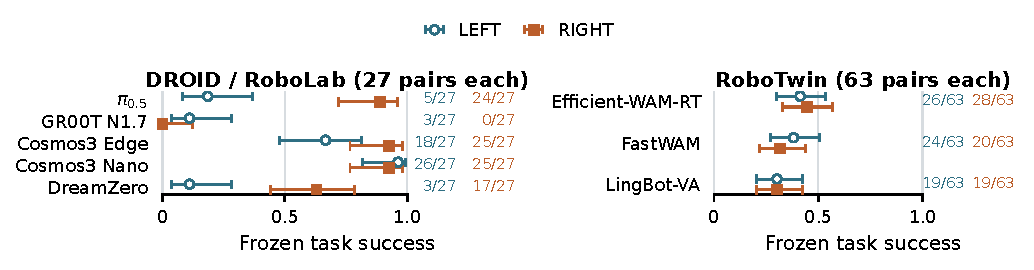
\includegraphics[width=0.98\textwidth]{figures/checkpoint_screen.pdf}
  \caption{\textbf{Directional task success varies across all eight checkpoint--arena rows.}
  Points show marginal \tokL{} and \tokR{} success with 95\% Wilson intervals.
  DROID/RoboLab uses 27 matched pairs per row and RoboTwin 63; their tasks and frozen predicates differ.
  This screen is separate from later intervention cohorts, and its intervals are descriptive rather than matched-pair tests.}
  \label{fig:screening}
\end{figure*}

% =============================================================================
% II. RELATED WORK
% =============================================================================
\section{Related Work}
\label{sec:related}

\tightparagraph{Generalist language-conditioned policies.}
Modern manipulation policies pair pretrained visual-language representations with expressive action decoders.
Representative systems include $\pi_0$ and $\pi_{0.5}$, which use flow-matching action models, OpenVLA, an open autoregressive alternative, and RT-2, which transfers web knowledge to control~\cite{black2024pi0,black2025pi05,kim2024openvla,brohan2023rt2}.
Hierarchical variants place a reasoning model above the controller and pass it natural-language subtasks~\cite{shi2025hirobot}.
Scale has expanded the tasks one policy can address, but it also makes a failed episode difficult to attribute: language interpretation, object localization, grasping, transport, release, and task scoring all lie on the same path to success.

\tightparagraph{Steerability and instruction following.}
A growing literature treats weak instruction following as the bottleneck and enriches the command interface.
CAST augments datasets with counterfactual language~\cite{glossop2025cast}; STEER relabels demonstrations to expose a low-level control interface~\cite{smith2025steer}; Steerable Policies train on subtask, motion, trace, and point commands~\cite{chen2026steerable}; InSight makes individual primitives addressable~\cite{wang2026insight}; and others steer a frozen policy at test time~\cite{jeong2026steering} or ask how steerability survives post-training~\cite{chen2026resteer,huang2026lockin}.
These methods address genuine failures of instruction following, but they rely on directional and relational success contrasts to certify that the failure was linguistic in the first place.

\tightparagraph{Diagnosing whether language is used.}
Counterfactual evaluation reduces attribution ambiguity by holding the visual input fixed while changing the instruction.
LIBERO-CF and Counterfactual Action Guidance examine cases in which visual evidence dominates a conflicting instruction~\cite{fang2026cag}, and recent analyses bound how far instruction following transfers to unseen phrasings~\cite{li2025confined}.
Steering protocols also report more than a single binary outcome: graded task progression against per-task rubrics~\cite{chen2026steerable}, a learned per-primitive progress channel~\cite{wang2026insight}, and success resolved by perturbation condition~\cite{jeong2026steering}.
These grade progress toward the command that was issued, a different quantity from a contrast between two commands sharing one reset and one sampling seed, and the difference is practical rather than an oversight: a matched contrast needs a resettable simulator~\cite{wang2026insight}.
Our question is complementary: when the objects are already fixed and the requested relation changes, does a \tokLR{} completion contrast uniquely diagnose language grounding?
Target contact, for example, verifies object selection but not whether the target reached the requested side of the reference.

\tightparagraph{Directional language and frozen task predicates.}
Grounding spatial and directional language into executable behavior long predates VLAs, and early systems already separated the referring expression, the spatial relation, and the executed path~\cite{kollar2010directions,tellex2011understanding}.
Current manipulation benchmarks instead retain a single frozen binary predicate, as they should; DROID and RoboTwin illustrate the data and simulation ecosystems used to train and test modern policies~\cite{khazatsky2024droid,mu2025robotwin}.
Such a predicate answers whether the task was completed in the evaluated scene distribution, but it can saturate at ceiling, collapse at floor, or hide large continuous placement changes.
We keep it as the final outcome and pair it with signed endpoint and requested-depth measurements and with interventions that vary language form and scene geometry separately.

% =============================================================================
% III. AUDIT DESIGN
% =============================================================================
\section{Audit Design}
\label{sec:method}

\tightparagraph{Minimal-pair token intervention.}
Literal prompt tokens appear in small capitals, \tokL{} and \tokR{}, while \emph{leftward} and \emph{rightward} denote physical directions in robot coordinates; a policy can track the token without preserving the direction it denotes.
For each reset $s_i$ we run a policy under prompts $\ell_i^L$ and $\ell_i^R$ that differ only in one opposite direction word, holding scene state, checkpoint, controller, environment seed, policy-sampling seed, action interface, and horizon fixed.
Both prompts therefore execute from an identical initial state, so any difference in the executed actions comes from the substituted word and nothing is left to adjust for.
We issue the instruction once at reset and leave it alone: no oracle actions, no prompt switching, and no language conditioned on progress.
DROID/RoboLab pairs the DROID Franka embodiment~\cite{khazatsky2024droid} with the RoboLab Isaac Sim environment~\cite{nvlabs2026robolab} and uses a Rubik's cube and bowl; RoboTwin~\cite{mu2025robotwin} uses a wooden block and playing-card box.
Both require placement and release in the requested relational region.

\tightparagraph{Evaluation corpus.}
Table~\ref{tab:corpus} lists the evaluated checkpoints; App.~\ref{app:provenance} records the released artifact identifier and exact revision behind each row.
Two are action-only VLAs and six are world-action models (WAM), which predict future observations alongside actions; all eight are driven through the same action interface and scored by the same frozen predicate.
Edge and Nano are the 4B and 16B policies of one Cosmos3 family~\cite{nvidia2026cosmos3}, so the rows are not fully independent.
The screen runs one matched-pair row per checkpoint and arena before any intervention: five DROID/RoboLab checkpoints at 27 matched pairs each and three RoboTwin checkpoints at 63, for 324 pairs, or 648 episodes.
The two arenas use different tasks and different success tests, so we report them separately throughout and do not pool them; the larger intervention cohorts state their own denominators.

\begin{table}[t]
  \centering
  \caption{Evaluated checkpoint--arena rows; short names in parentheses.}
  \label{tab:corpus}
  \small
  \begin{tabular}{@{}lcr@{}}
    \toprule
    Model (short name) & Class & Pairs \\
    \midrule
    \multicolumn{3}{l}{\emph{DROID/RoboLab: cube to the requested side of a bowl}}\\
    $\pi_{0.5}$ DROID~\cite{black2025pi05} & VLA & 27\\
    GR00T N1.7 DROID (GR00T)~\cite{bjorck2025gr00t} & VLA & 27\\
    Cosmos3 Edge Policy DROID (Edge)~\cite{nvidia2026cosmos3} & WAM & 27\\
    Cosmos3 Nano Policy DROID (Nano)~\cite{nvidia2026cosmos3} & WAM & 27\\
    DreamZero DROID (DreamZero)~\cite{ye2026dreamzero} & WAM & 27\\
    \midrule
    \multicolumn{3}{l}{\emph{RoboTwin: block to the requested side of a card box}}\\
    Efficient-WAM-RT~\cite{li2026efficientwam} & WAM & 63\\
    FastWAM~\cite{yuan2026fastwam} & WAM & 63\\
    LingBot-VA~\cite{hf2026lingbotva} & WAM & 63\\
    \bottomrule
  \end{tabular}
\end{table}

\tightparagraph{Behavioral measurements.}
Let $a^L_{1:T_L}$ and $a^R_{1:T_R}$ be the executed action sequences in a minimal pair, and let $y_i^L,y_i^R$ be the final target-minus-reference lateral offsets in robot coordinates, where positive is robot-left.
We report
\begin{align}
A_i &= \mathbb{1}\!\left[a^L_{1:T}\neq a^R_{1:T}\right],\ T{=}\min(T_L,T_R),\ D_i = y_i^L-y_i^R,\\
S_i^d &= \mathbb{1}[\text{frozen task predicate is satisfied for }d],\\
M_i^L &= y_i^L,\qquad M_i^R = -y_i^R.
\end{align}
$A_i$ uses bitwise inequality on the complete common executed prefix.
Positive $D_i$ means the requested endpoint ordering: within a pair the object came to rest further leftward under \tokL{} than under \tokR{}.
$S_i^d$ is task completion, and requested-side depth $M_i^d$ records how far the target moved toward the physical goal.

\tightparagraph{Calibrating $A_i$ against sampling noise.}
$A_i$ tests response, not semantics, and alone it is weak evidence: stochastic sampling makes two executions differ even under an unchanged prompt.
We therefore calibrate it on a single frozen observation, querying the policy without executing the robot so that no difference compounds through dynamics.
The diagnostic issues 336 action requests across six conditions (three DROID/RoboLab checkpoints crossed with the control and reflected scenes), each including a repeated request that must return identical output.
Its summary is a prompt-to-noise ratio: the \tokLR{} action difference at a matched seed over the root-mean-square difference between distinct seeds under an unchanged prompt.
A deterministic decoder makes that denominator zero, so for those rows we report the numerator alone rather than treating an undefined ratio as a small one.

\tightparagraph{Reference inversion.}
Base-frame prompts change the surface token and physical goal together; the reference-inversion control instead holds the physical relation fixed and changes its linguistic frame.
The base-frame prompts are ``Put the Rubik's cube to the left of the bowl.'' and ``Put the Rubik's cube to the right of the bowl.''
The inverted prompts are ``Place the Rubik's cube so that the bowl is to the right of the Rubik's cube.'' and the same sentence with \emph{left}.
All four name the cube as the object to place, so inversion changes the frame of the relational clause and not the manipulandum; the direction word flips while the intended physical relation does not.
The scorer, and the sign of $M$ for this control, follow the physical goal rather than the prompt text.
The $\pi_{0.5}$ study uses 341 resets in one symmetric DROID/RoboLab scene, with both forms of both physical goals sharing reset and sampling state, for 1,364 episodes on seeds disjoint from every scene-intervention cohort.

\tightparagraph{Geometry interventions.}
We use three scene interventions, each fixed in advance.
Reflection mirrors the centers of all movable objects about the robot sagittal plane while leaving the robot and fixed scene unchanged, and a seven-level sweep moves only the reference object laterally.
The symmetric-scene cohort drives an asymmetry metric to zero: the root-sum-square departure of the movable objects from bilateral symmetry about the robot midline, measuring midline objects from the midline itself and mirror-paired objects from each other's reflection, with position weighted at 10 per metre and orientation at 1 per radian.
The control layout scores 3.85 and the symmetric layout 0.00, within prespecified millimetre and half-degree tolerances, while robot, cameras, wrist mounting, reset posture, prompt, seed, and controller are identical across the two.
The symmetric package also changes which other objects are present, so it is not a position-only intervention and does not imply bilateral embodiment symmetry.
Every scene comparison first passes an endpoint-redirection positive control, asking whether the policy still moves its endpoint in the commanded direction in that row.
A row that fails it cannot show a scene change removing a directional gap, since nothing there was following the instruction; we report such rows and withhold the claim.

\tightparagraph{Scoring and inference.}
We do not relax the original task predicate.
Each episode receives exactly one outcome label, assigned in a fixed order: pick failed, transport failed, wrong side, release failed, or correct.
Every behavioral failure stays in its denominator.
Marginal binary rates use Wilson intervals, paired continuous contrasts use seed-clustered percentile bootstraps with 20,000 resamples and exact sign tests, and layout interactions use exact within-seed label permutations.
Absence claims require two one-sided equivalence tests (TOST) against prespecified margins, rather than nonsignificance~\cite{wilson1927interval,efron1994bootstrap,schuirmann1987tost}.
Prompts, seeds, success tests, target quantities, margins, and the failure-label order are all fixed before the runs they affect.
The released manifest records the exact seeds, checkpoint revisions, and freeze times behind every number reported here.

% =============================================================================
% IV. BASE-FRAME RESPONSE IS NOT SEMANTIC EQUIVALENCE
% =============================================================================
\section{Base-Frame Response Is Not Semantic Equivalence}
\label{sec:language}

\subsection{Base-frame minimal pairs}

All 324 base-frame minimal pairs across the eight rows execute different action sequences: 135 DROID/RoboLab pairs and 189 RoboTwin pairs.
Endpoint ordering is positive in $125/135$ and $128/189$ pairs, respectively.
These observations reject the narrow hypothesis that changing the direction token leaves control unchanged.
They do not show that the policy represents the relation independently of the wording, nor do they guarantee task completion.

The fixed-observation diagnostic of Sec.~\ref{sec:method} separates that response from sampling noise.
For $\pi_{0.5}$, prompt-induced action difference was about $4\%$ of cross-seed same-prompt variation but aligned across seeds.
For Nano the same ratio was $0.72$ under the control scene and $1.19$ after reflection: a much larger effect, and less consistently oriented.
DreamZero decodes deterministically, so the ratio is undefined for it rather than small and we report its action difference alone.
These open-loop rankings did not match closed-loop endpoint ordering, so action difference is a positive control, not a standalone grounding score.

\subsection{Reference inversion}

Reference inversion asks whether the same physical relation survives being expressed from the other object's frame.
Under inversion the direction word and the physical goal point opposite ways, which separates two behaviors that base-frame prompts cannot tell apart.
If the policy tracks the relation, the physical-\tokL{}-minus-physical-\tokR{} endpoint contrast should be positive.
If it tracks the direction word regardless of the sentence frame, the contrast should be negative, reaching $-23.28$\,cm if the base-frame response transferred unchanged.

Fig.~\ref{fig:inversion} shows neither.
Base-frame prompts separate the endpoints by $+23.28$\,cm (95\% CI $[21.89,24.56]$), whereas reference-inverted prompts yield only $+0.19$\,cm ($[-0.88,1.27]$).
The directional endpoint response therefore collapses under inversion: it provides neither reliable relation-consistent ordering nor evidence for token mirroring at the base-frame scale.
A collapse is also what we would see if the inverted phrasing were simply out of distribution, with the policy producing no coherent directional response instead of following either rule.
Our design does not separate that from a failure to transfer the relation; doing so would require inverted phrasings graded by familiarity while the physical goal is held fixed.
This conclusion is specific to endpoint direction, not all prompt sensitivity; all 682 base-frame/inverted physical-goal pairs execute different action traces.

\begin{figure}[t]
  \centering
  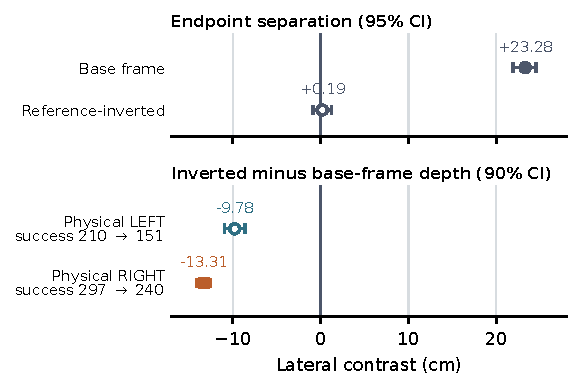
\includegraphics[width=0.98\columnwidth]{figures/reference_inversion.pdf}
  \caption{\textbf{Reference inversion collapses directional endpoint separation for $\pi_{0.5}$.}
  Top: physical-\tokL{}-minus-physical-\tokR{} endpoint separation with seed-clustered 95\% bootstrap intervals; positive is relation-consistent.
  Bottom: inverted-minus-base-frame requested-side depth with 90\% intervals; labels give base-frame-to-inverted success counts out of 341.
  This cohort's seeds are disjoint from those of the scene-intervention experiments.}
  \label{fig:inversion}
\end{figure}

Within each physical goal, inversion also reduces placement depth.
The inverse-minus-base-frame change is $-9.78$\,cm for physical \tokL{} (90\% CI $[-10.92,-8.59]$) and $-13.31$\,cm for physical \tokR{} ($[-14.07,-12.54]$); both intervals lie outside the prespecified $\pm4.15$\,cm equivalence margin.
Success falls from $210/341$ to $151/341$ for \tokL{} and from $297/341$ to $240/341$ for \tokR{}.
These rates also bound the competing reading that inversion silently changes which object is moved: the predicate scores placement of the cube, so a policy that switched to the bowl would fail almost everywhere, yet $151$ and $240$ of $341$ inverted episodes still satisfy it.
The corresponding changes, $-17.30$ and $-16.72$ percentage points, do not meet the prespecified $\pm15.56$-point equivalence criterion.
The inverse endpoint-ordering control also fails, so the semantic-equivalence claim is withheld.
Base-frame response is therefore insufficient evidence that a physical relation is preserved across reference frames.

% =============================================================================
% V. DIRECTIONAL COMPLETION TRACKS OBJECT GEOMETRY
% =============================================================================
\section{Directional Completion Tracks Object Geometry}
\label{sec:reflection}

Before any intervention we screen all eight rows of Table~\ref{tab:corpus}, and the directional gap differs sharply between them (Fig.~\ref{fig:screening}).
$\pi_{0.5}$ and DreamZero complete the task far more often under \tokR{} than \tokL{}, while GR00T barely completes it in either direction, $3/27$ against $0/27$, and is the only row whose small difference favors \tokL{}.
GR00T rarely grasps the cube at all: $49$ of its $54$ episodes end as pick failures, mostly with the cube nudged but never lifted, so completion has almost no room to vary with direction.
Nano is near ceiling under both prompts, and the three RoboTwin gaps are small.
The screen describes the rows we ran rather than ranking architectures.
The rest of this section asks how much of each gap the object layout accounts for.

\subsection{Position reflection}

Reflecting the centers of movable objects about the sagittal plane (Sec.~\ref{sec:method}) gives four conditions per checkpoint (two directions by two layouts) over 27 seeds, or 108 episodes for each of three DROID/RoboLab checkpoints.
The $\pi_{0.5}$ reflection cohort uses seeds disjoint from the screen, which is why Fig.~\ref{fig:screening} reports $5/27$ and $24/27$ where the control condition below has $4/27$ and $25/27$.
The primary outcome is the within-seed layout interaction in requested-side depth; success is secondary because binary outcomes can saturate by layout and direction.
Fig.~\ref{fig:reflection_scene} shows why with Nano, the checkpoint closest to the binary ceiling.

\begin{figure*}[t]
  \centering
  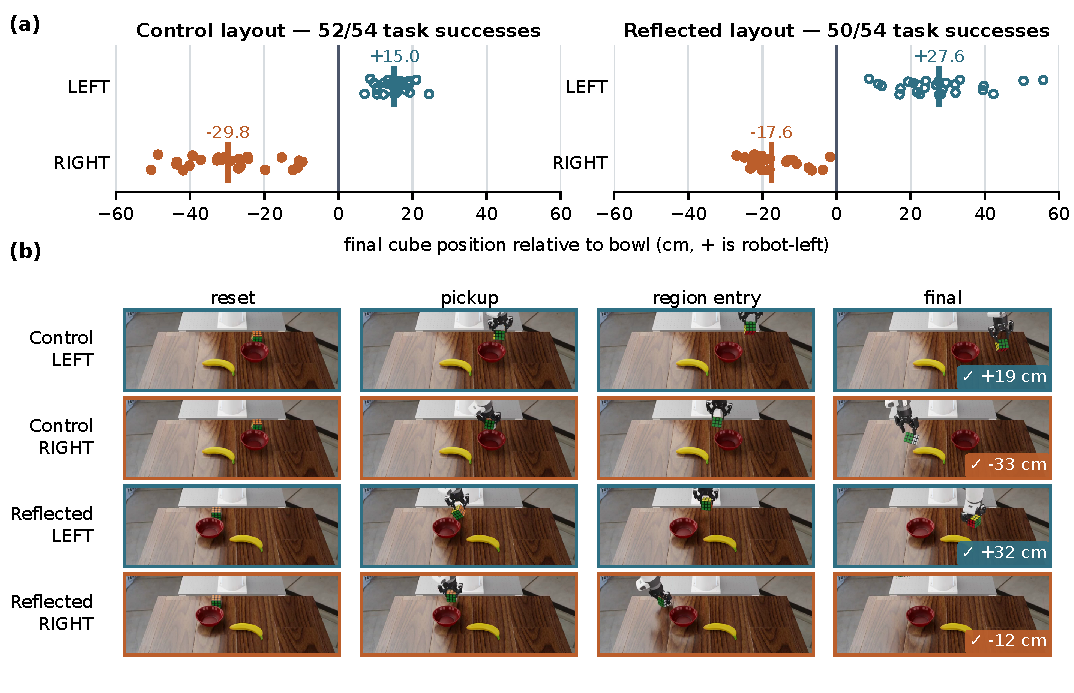
\includegraphics[width=0.98\textwidth]{figures/reflection_scene.pdf}
  \caption{\textbf{Reflecting movable-object positions moves the placement while the binary score stays at ceiling (Nano, 108 episodes).}
  (a) Final lateral cube position for every seed in the four conditions; bars mark their means and titles give task completion.
  The prompts still separate after reflection, by $45.3$\,cm against $44.8$\,cm in the control layout, but both distributions shift by about $12$\,cm, which is the requested-side depth interaction of $-24.8$\,cm reported below.
  Completion moves only from $52/54$ to $50/54$.
  (b) The executed rollout for the lowest released seed in each condition, sampled at that episode's logged events, with ticks marking the frozen predicate and numbers repeating the final signed offset.
  Robot-left appears toward the image right in this viewport, so the signed values rather than the images fix direction.
  Rollouts were selected by lowest released seed before any outcome was read.}
  \label{fig:reflection_scene}
\end{figure*}

\begin{figure*}[t]
  \centering
  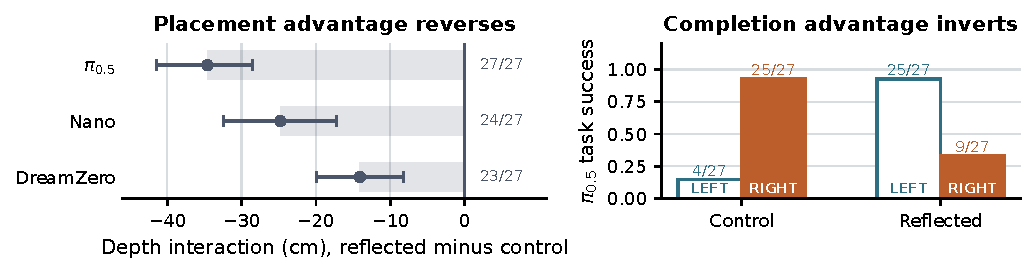
\includegraphics[width=0.98\textwidth]{figures/reflection_core.pdf}
  \caption{\textbf{Reflecting movable-object positions reverses placement advantage.}
  Left: reflected-minus-control interaction in requested-side depth, with seed-clustered 95\% bootstrap intervals; fractions give seeds with the negative interaction.
  Right: $\pi_{0.5}$ task completion in the independent reflection cohort.
  Nano is near a binary ceiling, while DreamZero changes from low control completion to near-ceiling reflected completion; their continuous depth interactions remain the quantity compared across checkpoints.}
  \label{fig:reflection}
\end{figure*}

As Fig.~\ref{fig:reflection} shows, requested-side depth reverses in every checkpoint: $-34.6$\,cm for $\pi_{0.5}$ (95\% CI $[-41.4,-28.5]$; $27/27$ seeds; $p=1.49\times10^{-8}$), $-24.8$\,cm for Nano ($[-32.4,-17.3]$; $24/27$; $p=4.92\times10^{-5}$), and $-14.1$\,cm for DreamZero ($[-19.9,-8.2]$; $23/27$; $p=3.11\times10^{-4}$).
For Nano and $\pi_{0.5}$, the estimated interactions in endpoint redirection are much smaller, $+0.5$\,cm and $-1.12$\,cm.
Both carry $p=.701$ because the exact sign test sees mirrored 15/12 and 12/15 splits over the same 27 seeds, not because the estimates agree; equivalence was not established, so we do not call redirection invariant.
The supported contrast is that placement changes far more than the estimated redirection interaction.

For $\pi_{0.5}$, binary completion itself inverts.
The control layout yields $4/27$ \tokL{} versus $25/27$ \tokR{} successes; reflection yields $25/27$ versus $9/27$.
The mean per-seed difference-in-differences on $\tokR{}$-minus-$\tokL{}$ completion, reflected minus control, is $-1.37$ on a $[-2,2]$ scale ($p=5.96\times10^{-8}$).
The checkpoint, prompts, seeds, controller, and robot are unchanged.
Under an unchanged frozen predicate, which direction $\pi_{0.5}$ completes more often is decided by which side the movable objects are on.

\subsection{A graded intervention and converging controls}
\label{sec:graded}

Reflection is a large intervention, so we also move the bowl across seven lateral positions while retaining the same Nano checkpoint and 15 matched seeds per level (210 episodes).
The requested-depth contrast changes gradually over the full support, with a slope of $1.12$ cm of depth per cm of reference displacement (95\% CI $[0.72,1.56]$); 13 of 15 seed-level slopes are positive (exact $p=.00739$).
A post hoc middle-five sensitivity is weaker: $0.49$ (95\% CI $[-0.04,0.97]$), with 11 of 15 positive slopes ($p=.118$).
We therefore claim a graded dependence across the seven tested positions, not an interior linear law.
The fitted zero crossing lies outside the tested support.

\begin{figure*}[t]
  \centering
  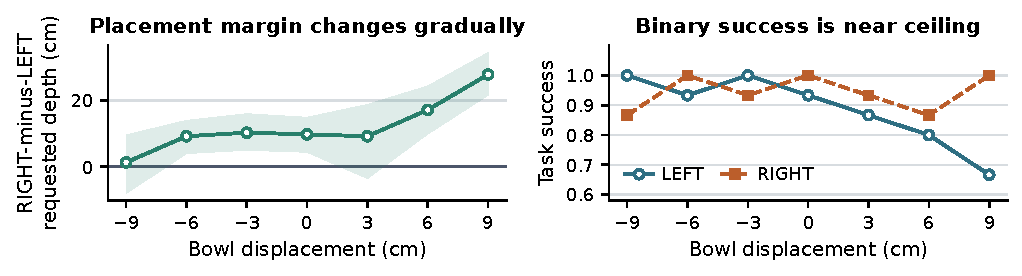
\includegraphics[width=0.98\textwidth]{figures/lateral_sweep.pdf}\\[3pt]
  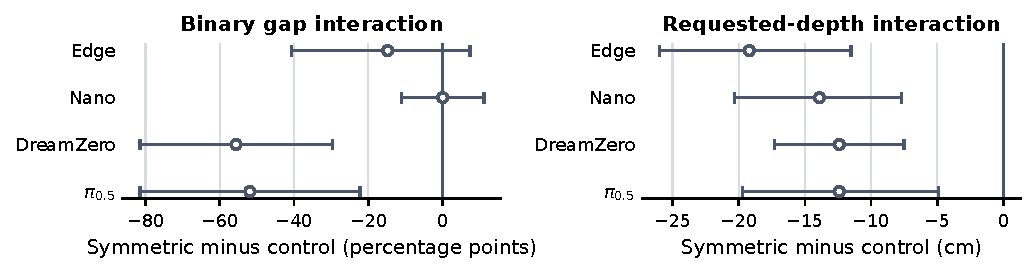
\includegraphics[width=0.98\textwidth]{figures/symmetry_core.pdf}
  \caption{\textbf{Two scene interventions, measured continuously and binarily.}
  Top: the directional placement contrast across the seven-position reference-object sweep, with mean \tokR{}-minus-\tokL{} requested-side depth and seed-clustered 95\% intervals on the left and frozen task success by requested direction on the right; each position contains 15 matched seeds.
  Bottom: symmetric-minus-control interactions in the matched 27-seed core of the positive-control-passing DROID/RoboLab cohort, with seed-clustered 95\% intervals; requested-depth disparity decreases in every checkpoint.
  In both interventions the continuous measure exposes variation that binary success compresses near ceiling, as for Nano.}
  \label{fig:scene}
\end{figure*}

Fig.~\ref{fig:scene} also shows why binary success alone is a weak diagnostic here: \tokL{} completion changes from $15/15$ to $10/15$, while \tokR{} stays close to ceiling.
Separate interventions point in the same direction.
Moving the target's start side changes success from $26/27$ versus $22/27$ to $23/27$ versus $27/27$ (interaction $+0.296$, $p=.0156$).
Swapping target and reference roles changes the depth contrast by $+13$\,cm (95\% CI $[6,21]$, $p=.00151$).
This role swap is the physical counterpart of the reference inversion in Sec.~\ref{sec:language}: there the sentence frame changes while the scene is fixed, here the objects exchange roles while the wording is fixed.
Finally, repeating policy sampling eight times in each of 27 fixed scenes gives 216 matched pairs per direction, with $41/216$ \tokL{} and $197/216$ \tokR{} successes: the gap is not an artifact of one draw.

% =============================================================================
% VI. A SYMMETRIC SCENE REDUCES THE GAP
% =============================================================================
\section{A Symmetric Scene Reduces the Gap}
\label{sec:symmetry}

The symmetric-scene cohort contains 4,096 episodes and 2,048 matched pairs across five checkpoint--arena rows.
The rows contribute unequally: 763 pairs for $\pi_{0.5}$ and 1,123 for Nano, whose endpoints carry 341 and 521 seeds, and 54 each for Edge, DreamZero, and FastWAM, evaluated at the two endpoints with the 27-seed matched core.
The intervention removes the object-layout residual (Sec.~\ref{sec:method}), but it replaces a whole scene package, including which other objects are present, rather than editing positions alone.
Four DROID/RoboLab checkpoints pass the endpoint-redirection positive control and support this comparison.
We did not include GR00T in this intervention, because it almost never completes the task in either direction; that is a scope decision, not a failed control.
FastWAM fails the control, so we report that row without claiming the scene change removed its gap.
A separate 108-episode RoboTwin cohort on LingBot-VA failed the same control at both layouts, so its geometry hypotheses were withheld under a decision rule fixed before the run and the checkpoint was not replaced; two of the three RoboTwin rows thus have a completed intervention that their own entry control gated out.
The $\pi_{0.5}$ seeds here are disjoint from the 341 used for reference inversion.

For $\pi_{0.5}$, the full 341-seed endpoints show the binary \tokR{}-minus-\tokL{} gap falling from 74.2 to 20.2 percentage points and the requested-depth gap from 17.0 to 5.75\,cm.
At the symmetric endpoint, their paired 90\% intervals are $[15.0,25.2]$ points against a prespecified $\pm15.56$-point margin and $[4.85,6.66]$\,cm against $\pm4.15$\,cm; neither is equivalent.
The separately defined matched 27-seed core estimates interactions of $-51.9$ points (95\% CI $[-81.5,-22.2]$, $p=.00786$) and $-12.4$\,cm (95\% CI $[-19.7,-4.9]$, $p=.00348$), respectively.
Base-frame redirection at the symmetric endpoint is $+23.9$\,cm, with $335/341$ positive pairs.

A separate layout supports the same conclusion without replacing the scene package, this cohort's main confound: centering the target and its reference on the robot midline and mirroring the existing clutter also drives the residual to zero, with the companion inventory unchanged.
Over its own 27 seeds and 54 episodes, $\pi_{0.5}$ still completed $25/27$ \tokR{} against $13/27$ \tokL{} requests (exact paired McNemar $p=.00183$), with requested-side depth $+6.18$\,cm ($[+3.29,+9.15]$) and endpoint redirection intact at $+23.77$\,cm; neither equivalence margin was met, and we keep the two residual estimates separate.

The matched core also shows why no single summary suffices (Fig.~\ref{fig:scene}).
DreamZero's observed binary gap changes from $+51.9$ to $-3.7$ points (interaction $-55.6$ points, $p=.00085$), bringing the measured gap near zero without establishing equivalence.
Nano has exactly zero binary interaction at ceiling ($p=1$), yet its 27-seed depth interaction is $-13.9$\,cm ($p=1.8\times10^{-4}$).
Edge is underpowered for its $-14.8$-point binary interaction, whose 95\% interval $[-40.7,+7.4]$ includes zero, while its depth interaction is $-19.2$\,cm (95\% CI $[-26.0,-11.5]$).

The same intervention changes failure composition, pooling directions over the 341 matched seed pairs.
Transport failures fall from 267 to 158, wrong-side failures from 41 to 7, pick failures from 1 to 0, and release failures from 2 to 0.
Those four classes and the success class exhaust each scene: the same 682 episodes carry 311 failures under the control layout and 165 under the symmetric package, with policy and prompt unchanged.

% =============================================================================
% VII. DISCUSSION
% =============================================================================
\section{Discussion}
\label{sec:discussion}

\tightparagraph{A directional gap is a property of a layout, not of a policy.}
Mirroring the movable objects reverses requested-side depth in all three reflection checkpoints, and it inverts $\pi_{0.5}$ completion from $4/27$ \tokL{} and $25/27$ \tokR{} to $25/27$ and $9/27$.
A graded reference-object sweep moves the same contrast continuously, and a symmetric scene reduces it in every checkpoint that still redirects on command.
Throughout, the evaluated policy, the prompts, and the seeds are unchanged.
So the quantity a directional score reports does not survive a change of layout, and it cannot be read as a fixed property of the checkpoint.

\tightparagraph{The decomposition separates a false failure from a false pass.}
A single binary contrast collapses two opposite errors of interpretation.
A \emph{false failure} occurs when a direction token redirects behavior, but the sampled scene makes one requested placement harder to complete; reflection, displacement, start-side, role-swap, and the symmetric scene all demonstrate this possibility.
A \emph{false pass} occurs when relation-consistent behavior under a familiar base-frame construction is treated as evidence of grounding even though the same physical goal does not transfer under reference inversion.
There, relation preservation and token mirroring predict opposite-signed endpoint contrasts, and the observed inverted contrast is near zero.
The four measurements and the inversion control tell these cases apart because they fail in different places: a ceiling can hide a 10--20\,cm change in placement quality, and an executed trace can change without expressing the intended relation.
The frozen predicate remains the correct final test of whether the robot completed the task.
It cannot, on its own, say why.

\tightparagraph{The controls discriminate rather than explain away.}
Removing the object-layout residual leaves $20.2$ points of the $\pi_{0.5}$ gap in place.
The paired 90\% interval $[15.0,25.2]$ excludes zero and is not contained in the prespecified $\pm15.56$-point margin, so equivalence fails.
We read that as a real checkpoint-specific residual rather than an inconclusive test, because the interval separates from zero instead of merely failing to fall inside the margin.
Scene controls that dissolved every directional gap would be indistinguishable from controls that merely degraded the measurement, which makes a surviving gap the more informative outcome.
It does not locate the residual in the policy.
The intervention zeroes one scene factor, and factors we did not equalize, such as per-side reachability given the remaining objects, could still produce what remains.

\tightparagraph{A minimum directional-grounding protocol.}
For relational placement, we recommend: (i) matched base-frame \tokLR{} prompts under identical reset and policy seeds; (ii) action distinctness and a direction-signed endpoint measure; (iii) continuous requested-side depth alongside the frozen success predicate; (iv) same-prompt repeats where stochasticity is material; (v) at least one matched scene intervention with a preserved endpoint-redirection positive control; and (vi) a reference inversion that preserves the physical goal.
Claims that an effect disappeared should rest on equivalence tests rather than a nonsignificant difference.

% =============================================================================
% VIII. LIMITATIONS
% =============================================================================
\section{Limitations}
\label{sec:limitations}

Our design trades external validity for control.
Exact state matching needs a resettable simulator, so hardware contact uncertainty and natural variation in human instructions remain untested, and the causal object-layout conclusions hold only for the DROID/RoboLab rows that pass the endpoint-redirection control; the RoboTwin rows screen behavior, not a cross-arena replication or refutation.
The task family is narrow as well: two named objects, one lateral relation, and one reference inversion on one $\pi_{0.5}$ checkpoint.

The interventions show the measured outcome depending on scene configuration without localizing the cause inside the model or robot.
Released material fixes each row's target-domain dataset but not episode membership or caption exposure, so we make no architecture-level or token-frequency claim and do not test whether the asymmetry is inherited from training data.
DreamZero's public demonstrations do include lateral placements referring to a bowl, so our task may sit closer to its demonstrated set than to the other rows'.
Two measurement gaps remain: we did not track reference-object displacement under inversion, though inverted success rates show the cube still moved (Sec.~\ref{sec:language}), and the fixed-observation diagnostic is action-space only.

% =============================================================================
% IX. CONCLUSION
% =============================================================================
\section{Conclusion}
\label{sec:conclusion}

The metrics currently used to judge steerability and responsiveness are incomplete.
A binary \tokLR{} success contrast answers four questions with one number: whether the instruction changed the executed actions, whether the change was oriented toward the requested relation, how far the object travelled toward it, and whether the frozen predicate was satisfied.
One number cannot separate them, so binary directional success does not isolate language grounding.
We report the four separately, as prompt-conditioned action change, signed endpoint ordering, continuous requested-side depth, and the frozen completion predicate, and we add two controls that a success score cannot supply on its own.
One is a matched scene intervention, read only where the policy still redirects its endpoint on command; the other is a reference inversion that holds the physical goal fixed while inverting the wording.
Both found a confound here.
Mirroring the movable objects reversed the favored direction for $\pi_{0.5}$, turning 4/27 \tokL{} and 25/27 \tokR{} into 25/27 and 9/27, and reference inversion cut the same checkpoint's endpoint separation from 23.3 to 0.2\,cm, in each case with the evaluated model unchanged.
Because a false failure and a false pass produce the same score, telling them apart takes measurements the score does not contain.
Each control is a scene transform or a prompt rewrite, so it can be added to an existing suite without retraining, new hardware, or any change to the success predicate.

% =============================================================================
% REFERENCES
% =============================================================================
\bibliographystyle{IEEEtran}
\bibliography{references}

% =============================================================================
% APPENDIX A. EVALUATED CHECKPOINT PROVENANCE
% =============================================================================
\appendices
\section{Evaluated Checkpoint Provenance}
\label{app:provenance}

Each row below is the exact artifact evaluated in this paper. The released manifest additionally records a content hash and the exact runtime identity for every row, and it records training-episode membership and caption exposure as undisclosed, which is why we make no token-frequency or pretraining-data claim anywhere in the paper.

\begin{table}[h]
  \centering
  \scriptsize
  \setlength{\tabcolsep}{3pt}
  \begin{tabular}{@{}ll@{}}
    \toprule
    Short name & Released artifact identifier and revision \\
    \midrule
    $\pi_{0.5}$ & \texttt{pi05\_droid\_jointpos\_polaris} \\
                & \texttt{v2a010-manifest-f5a56d9565f9381cc} \\
    GR00T & \texttt{nvidia/GR00T-N1.7-DROID} \\
          & \texttt{05e7cc97e40dbd33b0890c35cc0214fcb0547ab5} \\
    Edge & \texttt{nvidia/Cosmos3-Edge-Policy-DROID} \\
         & \texttt{3ea407af3e156c0af3b4bb6edd85842cc9a58777} \\
    Nano & \texttt{nvidia/Cosmos3-Nano-Policy-DROID} \\
         & \texttt{6706d7680581c255ff61e0f3bb49d90eac55c79e} \\
    DreamZero & \texttt{GEAR-Dreams/DreamZero-DROID} \\
              & \texttt{96ad344138c66e82536422432ad742f015784942} \\
    Efficient-WAM-RT & \texttt{jiajun0613/Efficient-WAM\_RoboTwin/} \\
                     & \texttt{Efficient-WAM-RT} \\
                     & \texttt{81280a79e8ac69dd6ffb9ce8698e00d122ec07fd} \\
    FastWAM & \texttt{yuanty/fastwam/} \\
            & \texttt{robotwin\_uncond\_3cam\_384.pt} \\
            & \texttt{139eebb6d90cdd9bdbbe465f72c6edc9ad5a518a} \\
    LingBot-VA & \texttt{lerobot/lingbot\_va\_robotwin} \\
               & \texttt{d1e1f93a84eaf9bca9880856fda800cc98cc8eaa} \\
               & \texttt{robbyant/lingbot-va-posttrain-robotwin} \\
               & \texttt{8c9dea8abbc5c91cc9e18bc3264b8915083bbe70} \\
    \bottomrule
  \end{tabular}
\end{table}

The $\pi_{0.5}$ row is an internal release rather than a public repository revision, so its recorded identifier is a manifest digest, abbreviated here and given in full in the released manifest. LingBot-VA is evaluated as a base checkpoint plus a RoboTwin post-training checkpoint, so both revisions are required to reproduce it.

\end{document}
